	\chapter{Building Blocks of Neural Networks}

	\section{Local Optimum and Saddle Points}
Non-convex functions have local minimums in addition to the global minimum (see \figurename~\ref{fig:complicatedlossfunction}).
 	\begin{figure}[h]
		\centering
		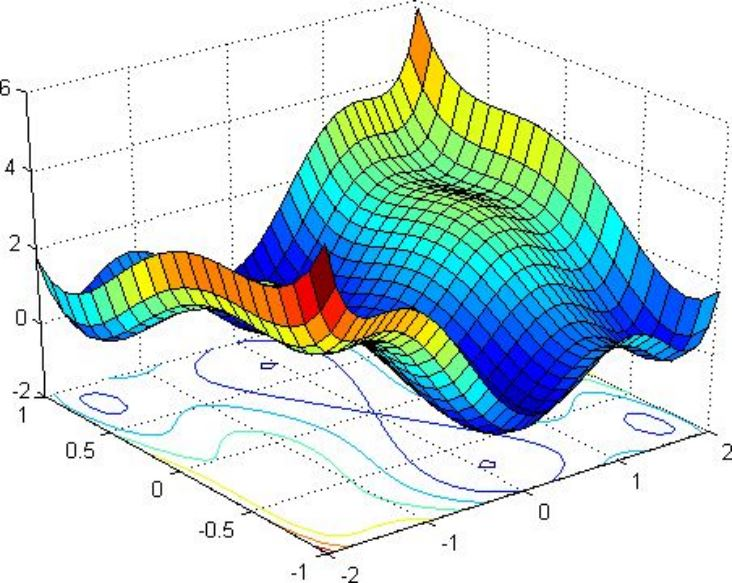
\includegraphics[height=2.0in]{complicatedlossfunction}
		\caption[Local minimums of a non-convex function]{Local minimums of a non-convex function.}
		\label{fig:complicatedlossfunction}
	\end{figure}

Saddle points, Hessian and long local furrows.  In multiple dimensions:
	\begin{bulletedlist}
		\item Some weights may have reached a local minima while others have not (see \figurename~\ref{fig:saddlepoint}).
		\item Some weights may have almost zero gradient.
		\item This all is characterized by a second derivative matrix called the Hessian, which is difficult to compute and invert.
		\item Different techniques try to approximate Hessian computation and inversion.
		\item Usually, they treat each weight independently and set learning rates for each differently.
		\item Examples: RMSprop, ADAM, Nesterov momentum.
	\end{bulletedlist}
 	\begin{figure}[h]
		\centering
		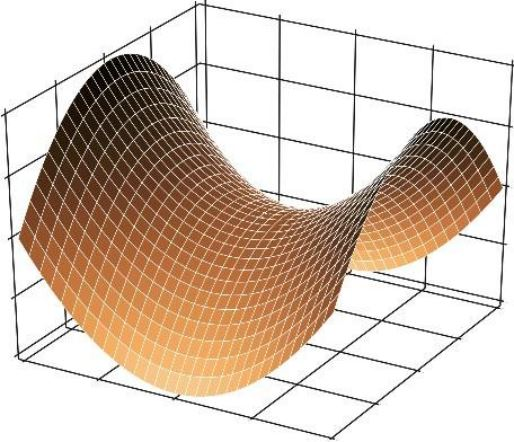
\includegraphics[height=2.0in]{saddlepoint}
		\caption[Saddle point]{Saddle point.}
		\label{fig:saddlepoint}
	\end{figure}


	\section{Other variants of Gradient Descent}
What is the need for advanced optimization?
	\begin{bulletedlist}
		\item Slow conversion rate.
		\item Gradient gets stuck in the local optima
	\end{bulletedlist}

Gradient descent optimization algorithms:
	\begin{bulletedlist}
		\item Gradient descent
		\item Stochastic gradient descent.
		\item Mini batch gradient descent.
		\item Adagrad (adaptive gradient descent).  Has individual learning rates for each dimension.  The entire learning rate decreases as optimization proceeds.  It does very well for convex problems.  For very non-convex surfaces, adagrad does not do well.  The learning rate can go to zero very fast, sometimes halting the optimization even before a local minimum is reached.
		\item Gradient descent with momentum.
		\item RMS prop (root mean square propagation).  Less aggressive than adagrad.  It is a decaying moving average (points in the past are weighted less than more recent points).
		\item Adam
	\end{bulletedlist}

In this course, we will be discussing RMSprop and Adam.

	\section{Stochastic Gradient Descent with Momentum}

	\begin{bulletedlist}
		\item Stochastic Gradient Descent is an optimization algorithm used in Machine Learning.
		\item During the training period to find the derivative loss function random data point is selected instead of whole data for each iteration.  For Example: A data set consists of 1000 data points and to calculate the derivative loss function it will be considering only one data point at a time.
		\item In SGD convergence to global minima happens very slowly as it will take a single record in each iteration during forward and backward propagation.
	\end{bulletedlist}
see \figurename~\ref{fig:stochasticgradientdescent}
 	\begin{figure}[h]
		\centering
		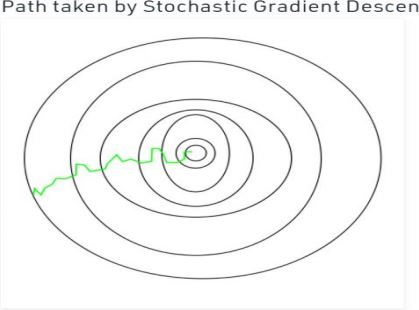
\includegraphics[height=2.0in]{stochasticgradientdescent}
		\caption[Stochastic gradient descent]{Stochastic gradient descent.}
		\label{fig:stochasticgradientdescent}
	\end{figure}

	\begin{bulletedlist}
		\item To overcome the noisy data produced by the Mini batch Gradient descent there is another variant of Gradient Descent called Gradient descent with momentum which will smoothen the noisy data.
		\item Gradient Descent with Momentum uses exponentially weighted averages of gradients over the previous iteration to stabilize the convergence (see \figurename~\ref{fig:stochasticgradientdescent}).
	\end{bulletedlist}
 	\begin{figure}[h]
		\centering
		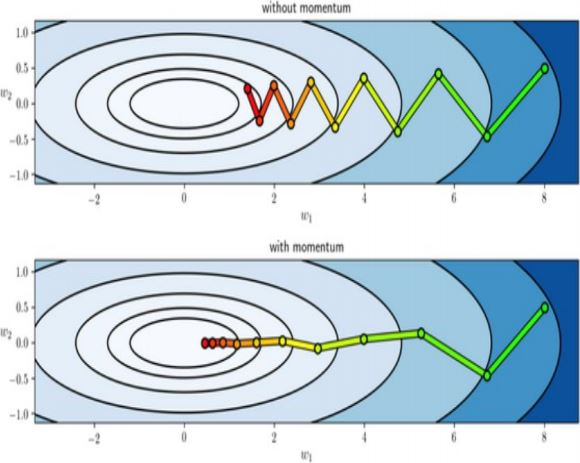
\includegraphics[height=2.0in]{stochasticgradientdescentmomentum}
		\caption[Stochastic gradient descent with momentum]{Stochastic gradient descent with momentum.}
		\label{fig:stochasticgradientdescentmomentum}
	\end{figure}


	\section{RMSprop}

	\begin{bulletedlist}
		\item RMSprop optimization is termed as root mean squared propagation optimization technique.
		\item It is a gradient based optimization technique used in training a neural network.
		\item Gradients of very complex functions like neural networks have a tendency to either vanish or explode as the data propagates through the function.
		\item RMSprop deals with this issue by using a moving average of squared gradients to normalize the gradient.
		\item RMSprop is an adaptive learning algorithm that tries to improve AdaGrad. Instead of taking the cumulative sum of squared gradients like in AdaGrad, it takes the ``exponential moving average.''
		\item This balances the step size, decreasing the step for large gradients to avoid exploding and increasing the step for small gradients to avoid vanishing.
		\item RMSprop is preferred over gradient descent because it has a very good convergence speed towards the minima of the cost function.
	\end{bulletedlist}

	\subsection{How it Works}
Please reference \figurename~\ref{fig:rmsprophowitworks} for the following:
	\begin{bulletedlist}
		\item Here Vdw and Vdb are the exponential averages of squares of gradients.
		\item $\beta$ is a hyperparameter and W is the weight term.
		\item dw2 and db2 are the second-order derivative of the cost function with respect to the weight and bias respectively.
		\item $\alpha$ is the learning rate. In RMSprop learning rate is not a hyperparameter.  It is managed by the algorithm itself, instead of being tuned.
		\item $\epsilon$ epsilon is the additive term.  It just ensures that the denominator does not get equal to zero when Vdb or Vdw becomes equal to zero.  Ideally, its value is 10-8.
		\item Ideally, dw is small and db is high. Hence step size of w increases(divided by a smaller number) and that of b decreases(divided by a larger number).  Due to this the convergence in the direction of weight increases in RMSprop.
	\end{bulletedlist}
 	\begin{figure}[h]
		\centering
		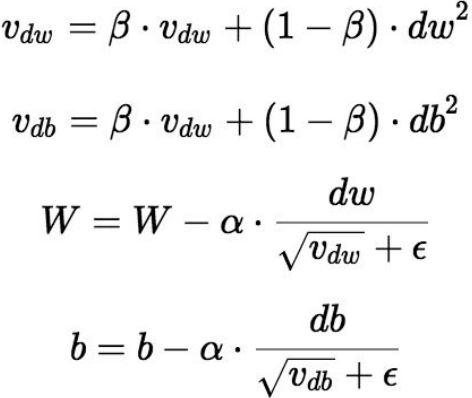
\includegraphics[height=2.0in]{rmsprophowitworks}
		\caption[Root mean square propagation equations]{Root mean square propagation equations.}
		\label{fig:rmsprophowitworks}
	\end{figure}

	\subsection{Estimating Moments of the Gradient}

	\begin{bulletedlist}
		\item In stochastic gradient descent with momentum, we compute the first moment of the gradient ($g_t$) given as $m_t$ in the below diagram.
		\item In RMSprop we compute the second moment of the derivative. It is given as $V_t$ in the diagram.
		\item $\beta_1$ and $\beta_2$ are tunable hyperparameters of the algorithm.
	\end{bulletedlist}

In \equationname{}s~\ref{eq:firstmoment} and~\ref{eq:secondmoment} $m_t$ is the first moment (mean) of the gradient.  While $V_t$ is the second moment of the gradient.
	\begin{align}
		m_t &= \beta_1 m_{t-1} + \left( 1-\beta_1 \right) g_t   \label{eq:firstmoment} \\
		v_t &= \beta_2 v_{t-1} + \left( 1-\beta_2 \right) g_t^2 \label{eq:secondmoment}
	\end{align}

	\subsection{Why RMSprop Enhances Convergence Speed}
	\begin{bulletedlist}
		\item The generic problem in traditional optimization algorithms like gradient descent is the speed of convergence. The gradient in the direction of weight is low and in the direction of bias is high.
		\item Let us understand this in the dimensions of weights and bias of gradient descent.  In an ideal scenario, we need a high convergence speed in the direction of weight(or horizontal direction) and a slow speed in the direction of bias (vertical direction) in gradient descent.
		\item In GD we have uncontrolled steps in both directions.  This hinders the freedom of choosing a bigger learning rate (due to the risk of overshooting minima) while attempting to speed up the convergence.
		\item While using RMSprop, we dampen the movement in the direction of bias and in parallel speed up the same in the direction of weight.  This helps to solve the problem in two ways:
		\begin{bulletedlist}
			\item It speeds up the convergence in the direction of weight.
			\item It slows down the convergence speed in the direction of bias.
		\end{bulletedlist}
	\end{bulletedlist}

	\section{Adam}
``Adam'' stands for ``adaptive moments.''  Adam (2014) is RMSprop (learning rate) and stochastic gradient descent with momentum (solver/optimizer).  Adam is fast but comes at a small price. Stochastic gradient descent with momentum can typically find better minimums than Adam.

	\begin{bulletedlist}
		\item Adam can be defined as the merger of RMS prop and SGD with momentum.
		\item Like RMSprop, it utilizes the squared gradients to scale the learning rate, and similarly, like SGD with momentum, it uses the moving average of the gradient as an alternative to the gradient itself.
		\item Adam utilizes the estimations of the first and second moments of the gradient to adapt the learning rate for each weight in the neural network.
		\item The first moment is the mean and the second moment is not centered variance, i.e.\ during the calculation of variance, we don't subtract the mean.
	\end{bulletedlist}

The first and second moments are seen in \equationname{}s~\ref{eq:firstmoment} and~\ref{eq:secondmoment}, respectively.  \equationname{}s~\ref{eq:biascorrectedfirstmoment} and~\ref{eq:biascorrectedsecondmoment} are the bias corrected estimates of the first and second moments, respectively.

	\begin{align}
		\hat{m}_t     &= \frac{m_t}{1-\beta_1^t }    \label{eq:biascorrectedfirstmoment} \\
		\hat{v}_t     &= \frac{v_t}{1-\beta_2^t} \label{eq:biascorrectedsecondmoment}    \\
		\theta_{t+1}  &= \theta_t - \frac{\eta \hat{m}_t}{\sqrt{\hat{v}_t+\epsilon}}
	\end{align}

	\begin{bulletedlist}
		\item Adam optimizer is termed as Adaptive moment estimation optimizer.
		\item Algorithms like Stochastic gradient descent with momentum, RMSprop, and Adam's optimizer are similar in performance but Adam has a slight edge over the others due to the
bias correction performed in Adam.
		\item In reality, Adam optimizer is a combination of Stochastic gradient descent with momentum and the RMSprop.  In Adam, the learning rate becomes a tunable hyperparameter while in RMSprop it is an adaptive parameter.
		\item Adam optimizer can be explained in below three steps:
		\begin{numberedlist}
			\item Estimating moments of the gradient.
			\item Bias correction step.
			\item Updating the weights.
		\end{numberedlist}
	\end{bulletedlist}

	\subsection{Bias Correction Step}
	\begin{bulletedlist}
		\item In Adam's optimization, the most crucial step is the bias correction part.  In RMSprop we initiate the momentum terms(mt and vt )with 0 which is a bias. In Adam optimization, the bias correction step makes it independent of the initial value.
		\item The below steps are called bias correction steps.
		\item The ideal value of $\beta_1$ is 0.9 while that of $\beta_2$ is 0.999.
	\end{bulletedlist}

	\subsection{Updating the Weights}
Now finally the weights are updated as follows

	\section{Weight initialization and its Techniques}

What is Weight Initialization?
	\begin{bulletedlist}
		\item Weight Initialization is a procedure to assign weights to a neural network with some small random values during the training process in a neural network model.
	\end{bulletedlist}

\vspace{\baselineskip}
\noindent Why do we need Weight Initialization?
	\begin{bulletedlist}
		\item The purpose of using the weight initialization technique is to prevent the neural network from exploding or vanishing gradient during the forward and
backward propagation. If either occurs, the neural network will take a longer time to converge.
		\item For example, very large weights will push the activation functions like Sigmoid out to the edges where the gradient is essentially zero.
		\item You want the variance to sum to a constant.  If it collapses to zero, the same weights (no variance) are used across all nodes of the layer.  A single node could capture the same information.
	\end{bulletedlist}


 	\begin{figure}[h]
		\centering
		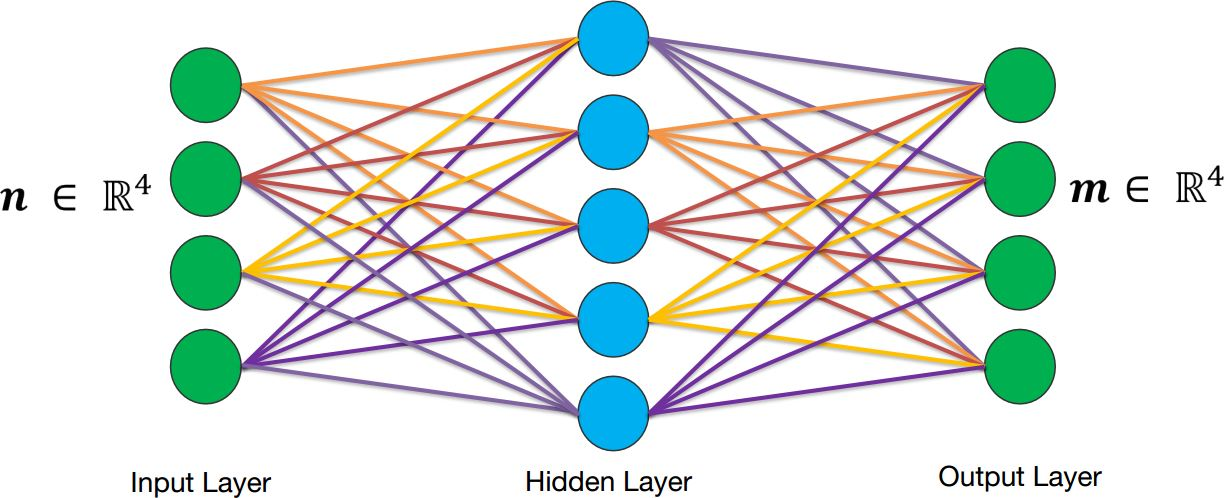
\includegraphics[height=2.5in]{weightinitialization}
		\caption[Weight initialization for neural networks]{Weight initialization for neural networks.}
		\label{fig:weightinitialization}
	\end{figure}

	\begin{bulletedlist}
		\item {\bfseries Initialize all weights with 0}:  Your network will not learn as all the weights are the same.
		\begin{bulletedlist}
			\item This makes your model equivalent to a linear model.
			\item When you set all weights to 0, the derivative with respect to loss function is the same for every w in every layer, thus, all the weights have the same values in the subsequent iteration.
			\item This makes the hidden units symmetric and continues for all the n iterations you run.
			\item Thus setting weights to zero makes your network no better than a linear model
		\end{bulletedlist}
		\item {\bfseries Initialize all weights with large numbers}:  The activation functions becomes a linear combination of large numbers.  Activation functions like Sigmoid have gradients close to zero at the extreme edge, therefore the model cannot learn.
		\item {\bfseries Initialize with random numbers}: Works okay for small networks (similar to our two-layer MNIST classifier), but it may lead to distributions of the activations that are not homogeneous across the layers of the network.
		\begin{bulletedlist}
			\item Initializing weights randomly, following standard normal distribution (np.random.randn(n, n-1) in Python) while working with a (deep) neural network can potentially lead to 2 issues - vanishing gradients or exploding gradients.
			\item The variance drops in the deeper layers.
		\end{bulletedlist}
	\end{bulletedlist}

	\subsection{Vanishing Gradients}
In the case of deep networks, for any activation function, abs(dW) will get smaller and smaller as we go backward with every layer during back propagation.  The earlier layers are the
slowest to train in such a case.

The weight update is minor and results in slower convergence.  This makes the optimization of the loss function slow.  In the worst case, this may completely stop the neural network from training further.

 	\begin{figure}[h]
		\centering
		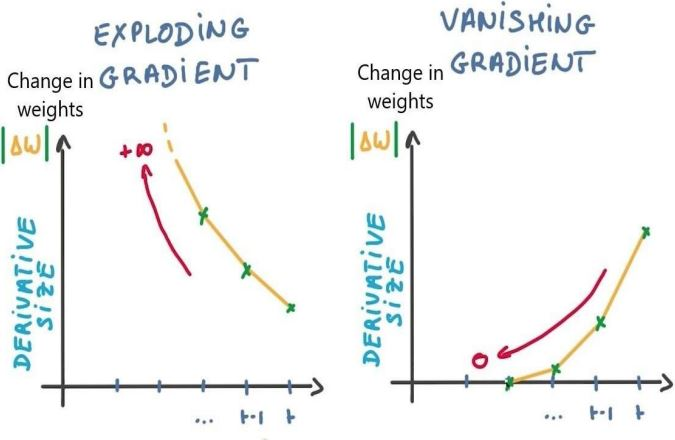
\includegraphics[height=2.5in]{vanishingandexplodinggradients}
		\caption[Vanishing and exploding gradients]{Vanishing and exploding gradients.}
		\label{fig:vanishingandexplodinggradients}
	\end{figure}

	\subsection{Exploding Gradients}
This is the exact opposite of vanishing gradients.  Consider you have non-negative and large weights and small activations A (as can be the case for sigmoid(z)).

This may result in oscillating around the minima or even overshooting the optimum again and again and the model will never learn!

Another impact of exploding gradients is that huge values of the gradients may cause number overflow resulting in incorrect computations or introductions of NaN's.  This might also lead to the loss of taking the value NaN.

	\subsection{Weight Initialization Techniques}
 	\begin{figure}[h]
		\centering
		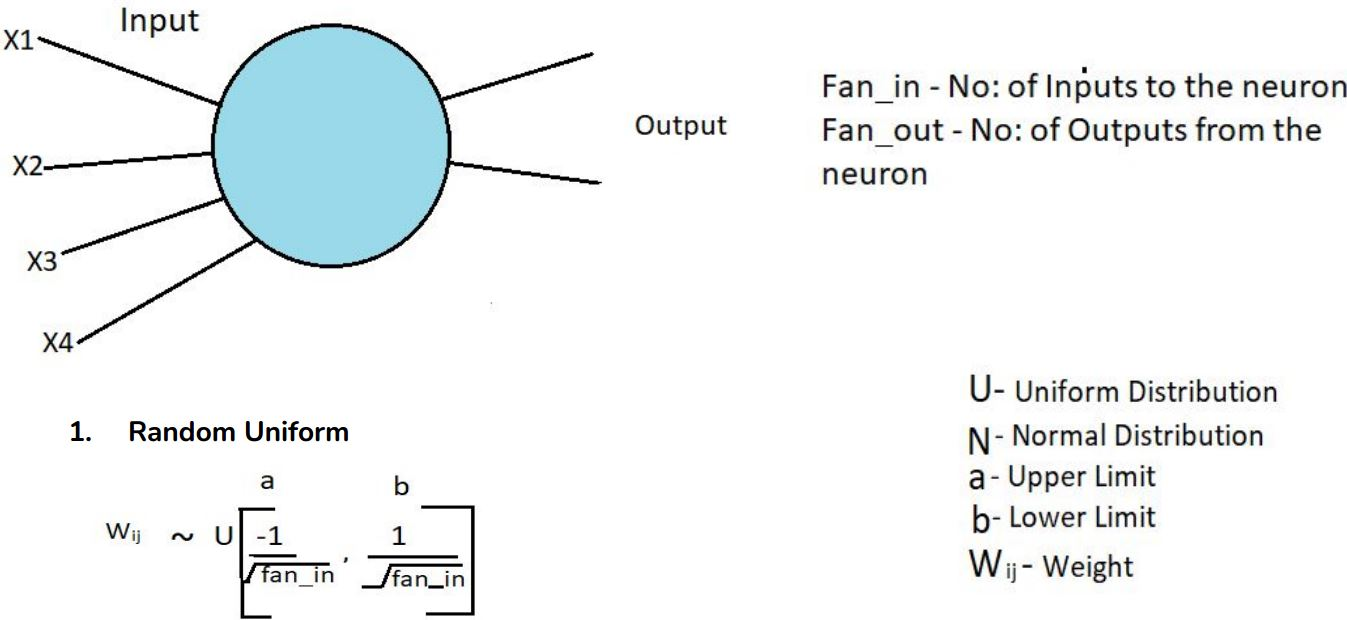
\includegraphics[height=3in]{weightinitialization1}
		\caption[Neural network weight initialization]{Neural network weight initialization.}
		\label{fig:weightinitialization1}
	\end{figure}

	\begin{bulletedlist}
		\item Random Uniform
		\item {\bfseries Xavier Initialization}
		\begin{bulletedlist}
			\item We want to initialize the weights with random values that are not ``too small'' and not ``too large'' (see \figurename{}).
			\item Weights are chosen based on the number of nodes in the previous layer.
			\item Today, this means take all weights, sample from a normal distribution, adjusted for number of nodes from previous layer.
		\end{bulletedlist}
	\end{bulletedlist}

	\begin{figure}[tbp]
		\begin{minipage}[t]{0.475\textwidth}
			\centering
			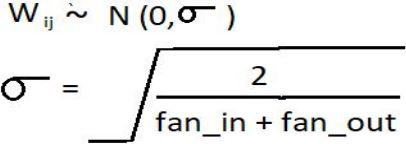
\includegraphics[height=0.75in]{xaviernormal}
			\caption[Xavier normal initialization]{Xavier normal initialization.}
			\label{fig:xaviernormal}
		\end{minipage}
		\hfill
		\begin{minipage}[t]{0.475\textwidth}
			\centering
			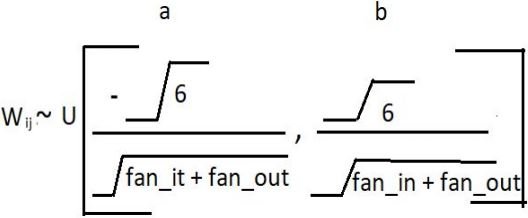
\includegraphics[height=1.0in]{xavieruniform}
			\caption[Xavier uniform initialization]{Xavier uniform initialization.}
			\label{fig:xavieruniform}
		\end{minipage}
	\end{figure}

	\begin{figure}[tbp]
		\begin{minipage}[t]{0.475\textwidth}
			\centering
			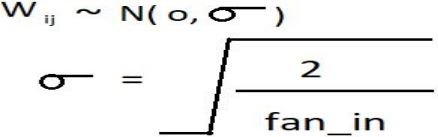
\includegraphics[height=0.65in]{henormal}
			\caption[HE normal initialization]{HE normal initialization.}
			\label{fig:henormal}
		\end{minipage}
		\hfill
		\begin{minipage}[t]{0.475\textwidth}
			\centering
			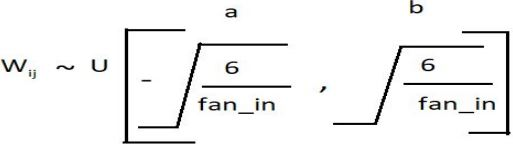
\includegraphics[height=0.8in]{heuniform}
			\caption[HE uniform initialization]{HE uniform initialization.}
			\label{fig:heuniform}
		\end{minipage}
	\end{figure}

HE is used for activation functions that cut off half of the weights (ReLU), you double the weights to account.

	\subsection{Best Practices}
Which is Good?  Weight initialization techniques for different activation functions:

	\begin{table}
        \centering
        \caption[Pairing activation functions with weight initialization techniques]{Pairing activation functions with weight initialization techniques.}
        \label{tab:activationfunctionsandweightinitialization}
		\begin{tabular}{|p{0.5\qandatextwidth-2\tabcolsep}|p{0.5\qandatextwidth-2\tabcolsep}|} \hline
				\tablecolumnheadervlinesone{Activation Function} & \tablecolumnheadervlinestwo{Weight Initialization Technique} \\ \hline
				Relu, Leaky Relu &
				HE Initialization \\ \hline
				Sigmoid, TanH &
				Xavier Initialization \\ \hline
		\end{tabular}
	\end{table}

	\subsection{Continued Research}
Proper Initialization is an active area of research:

\researchreference{Understanding the difficulty of training deep feed forward neural networks}{by Glorot and Bengio, 2010}
\researchreference{Exact solutions to the nonlinear dynamics of learning in deep linear neural networks}{by Saxe et al, 2013}
\researchreference{Delving deep into rectifiers: Surpassing human-levll performance on ImageNet classification}{by He et al., 2015}
\researchreference{Data-dependent Initializations of Convolutional Neural Networks}{by Kr{\"a}henb{\"u}hl et al., 2015}
\researchreference{All you need is a good init}{by Mishkin and Matas, 2015}
\researchreference{Centered Weight Normalization in Accelerating Training of Deep Neural Networks}{by Huang et al., 2017}
\researchreference{Adjusting for Dropout Variance in Batch Normalization and Weight}{Initialization: by Hendrycks et al., 2017}

	\section{Over Fitting in Neural Networks}

	\begin{bulletedlist}
		\item Neural networks are prone to over fitting because of the larger number of parameters.
		\item ANN is able to model higher order and complex functions which makes it more prone to over fitting.
	\end{bulletedlist}

 	\begin{figure}[h]
		\centering
		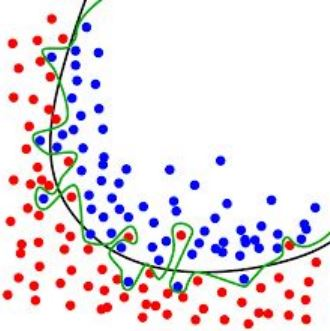
\includegraphics[height=2.25in]{neuralnetworksoverfitting}
		\caption[Over fitting in neural networks]{Over fitting in neural networks.}
		\label{fig:neuralnetworksoverfitting}
	\end{figure}

	\section{Regularization}
{\bfseries The solution to over fitting is regularization.}

A fully connected layer occupies most of the parameters, and hence, neurons develop co-dependency amongst each other during training which curbs the individual power of each neuron leading to over-fitting of the training data.

How could this possibly be a good idea?  It forces the network to have a redundant representation.  Another interpretation is that a dropout is an approach to regularization in neural networks which helps to reduce interdependent learning amongst the neurons.

	\begin{figure}[tbp]
		\begin{minipage}[t]{0.475\textwidth}
			\centering
			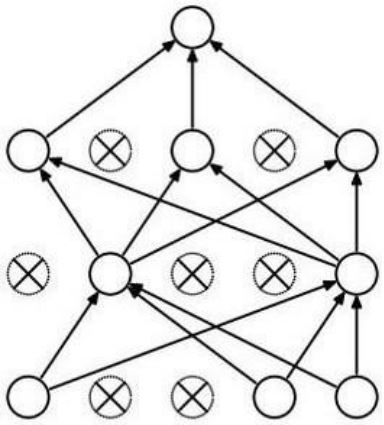
\includegraphics[height=1.25in]{dropoutredundent1}
			\label{fig:dropoutredundent1}
		\end{minipage}
		\hfill
		\begin{minipage}[t]{0.475\textwidth}
			\centering
			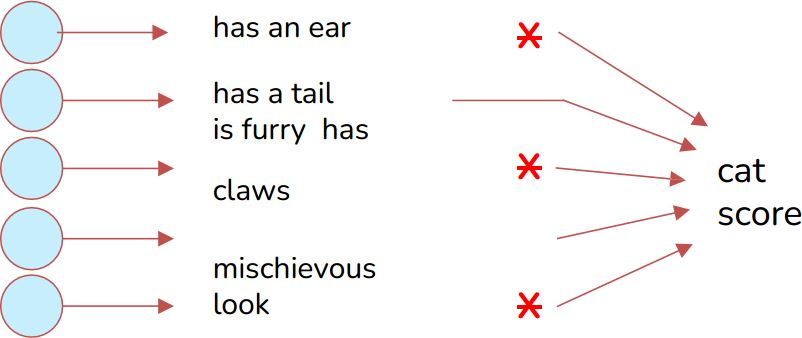
\includegraphics[height=1.25in]{dropoutredundent2}
			\label{fig:dropoutredundent2}
		\end{minipage}
		\caption[Use of drop out to prevent over fitting]{Use of drop out to prevent over fitting.}
	\end{figure}

At test time all neurons are always ON.  We must scale the activations so that for each neuron: output at test time = expected output at training time.

A $\lambda$ parameter adds a penalty to the loss function prevent large weights.

	\subsection{Early Stopping}
	\begin{bulletedlist}
		\item Early stopping is a technique similar to cross-validation where a part of training data is kept as the validation data. When the performance of the validation data starts worsening, the model will immediately stop the training.
		\item We usually reduce over fitting by observing the training/validation accuracy gap during training and then stop at the right point.
		\item In the given in \figurename~\ref{fig:regularzationearlystopping}, the model will stop training at the dotted line since after that our model will start over fitting on the training data.
	\end{bulletedlist}

 	\begin{figure}[h]
		\centering
		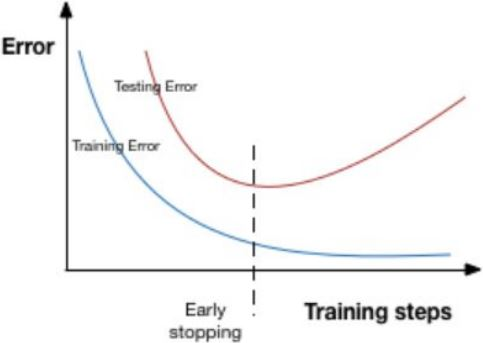
\includegraphics[height=2.25in]{regularzationearlystopping}
		\caption[Preventing over fitting by stopping when testing error starts increasing]{Preventing over fitting by stopping when testing error starts increasing.}
		\label{fig:regularzationearlystopping}
	\end{figure}

	\subsection{L2 and L1 Regularization}
	\begin{plainlist}
		\item L1
		\begin{bulletedlist}
			\item Lasso (least absolute shrinkage and selection operator)
			\item $\sum \left| w_i \right|$
			\item Sets some weights to zero (causing them to drop out, reduces connection between nodes) which is why it is referred to as a selection operator.
		\end{bulletedlist}
		\item L2
		\begin{bulletedlist}
			\item Ridge
			\item $\sum \left( w_i \right)^2$
			\item Reduces some weights to very small.
		\end{bulletedlist}
	\end{plainlist}

	\vspace{\baselineskip}
	\begin{bulletedlist}
		\item {\bfseries Penalty terms}: L1 regularization uses the sum of the absolute values of the weights, while L2 regularization uses the sum of the weights squared.
		\item {\bfseries Feature selection}: L1 performs feature selection by reducing the coefficients of some predictors to 0, while L2 does not.
		\item {\bfseries Computational efficiency}: L2 has an analytical solution, while L1 does not.
		\item {\bfseries Multi-collinearity}: L2 addresses multi-collinearity by constraining the coefficient norm.
	\end{bulletedlist}

	\subsection{L2 Regularization}
	\begin{bulletedlist}
		\item Due to the addition of the regularization term, the weights decrease because it assumes that a neural network with a smaller weight leads to
a simpler model. Therefore, it will also reduce the over fitting problem to quite an extent.
		\item Weight updation equation with regularization term is given in fig (b).
		\item If the learning rate is high difference in (1-nl) will be low and weights will go down.
		\item If the learning rate is low the difference in (1-nl) will be high and weights will be high.
	\end{bulletedlist}

	\begin{equation}
		W_{ij} - \frac{n\nabla\left(L\right)}{\nabla W_{ij}}
	\end{equation}
	\begin{equation}
		W_{ij}\left(1-nl\right) - \frac{n\nabla\left(L\right)}{\nabla W_{ij}}
	\end{equation}
	\begin{mathwhere}[0.75in]
		\mathdefitem{n}{the learning rate;}
		\mathdefitem{l}{the regularization parameter;}
		\mathdefitem{(1-nl)}{weight decay.}
	\end{mathwhere}

	\subsection{Data Augmentation}
Generating new data to supplement the existing data.  For example, add noise to images, rotate images, change color of images.

	\subsection{Dropout Regularization}
	\begin{bulletedlist}
		\item During \textbf{training}, randomly set some neurons to zero in the forward pass.
		\item During \textbf{testing}, all neurons are on.
		\item Because of the different number of neurons on during training and testing, the weights must be scaled.
		\item Forces the nodes to start to train separately, preventing some nodes from becoming strong and some becoming weak.
		\item You can implement drop out on any layer except the output.
		\item Builds some redundancy for situations where some input is not present, et cetera.
		\item Effectively creates several smaller networks that are combined in the end.
		\item Can help prevent co-adapting (nodes in one layer introduce an error and nodes in another layer correct it).
		\item With dropout, nodes are getting less input than in the full model, therefore weights must be scaled to adjust for the increase in input.  You can scale during training or during testing.
		\begin{bulletedlist}
			\item Regular dropout: scaling during testing.
			\item Inverse dropout: scaling during training.
		\end{bulletedlist}
		\item Dropout probabilities:
		\begin{bulletedlist}
			\item Input layer: A dropout probability of 0.8 works well (use 80\% of input).
			\item Hidden layers: A dropout probability of 0.5 works well.
			\item Output layer: Don't use dropout.
		\end{bulletedlist}
	\end{bulletedlist}

 	\begin{figure}[h]
		\centering
		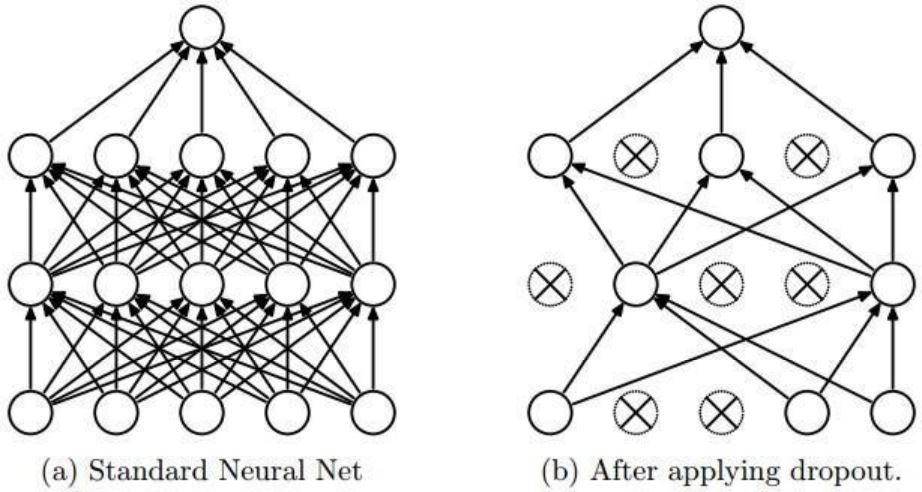
\includegraphics[height=2.25in]{dropout}
		\caption[Before and after applying drop out in a neural network]{Before and after applying drop out in a neural network.}
		\label{fig:dropout}
	\end{figure}

	\subsubsection{Guidelines for Dropout}
	\begin{bulletedlist}
		\item The choice of which units to be dropped is random.
		\item The Dropout method is similar to the Random Forest technique in selecting the random features for the model building.
		\item What should be the Dropout ratio in a neural network is a hyperparameter. The dropout ratio (p) is between 0<=p<=1. Whenever a deep neural network is over fitting the (p) value should be high.
		\item A good value for the dropout ratio in the hidden layer is 0.5-0.8.
		\item The Dropout technique is applied to the training data, during prediction on test data all the neurons will be fully connected and one additional work is done during prediction is the dropout ratio (p) with be multiplied with weights (w) in every layer.
	\end{bulletedlist}

	\section{Noise in Neural Networks}
	\begin{bulletedlist}
		\item Training a neural network with smaller data sets may be prone to over fit the model so adding some noise during the training process can make the model more robust and reduce generalization error.
		\item Noise can be added in various formats. It is mainly added to inputs, weights, activation functions, and even gradients.
		\item The commonly used noise for training is Gaussian noise and it is mainly added to the input variables. Gaussian noise is simply termed to be a noise with a mean of zero and standard deviation of one and adding this noise to the inputs is termed as jitter.
		\item Here the amount of noise to be added is a hyperparameter.
	\end{bulletedlist}

	\section{Batch Normalization}

	\begin{bulletedlist}
		\item Batch normalization is a technique for improving the performance and stability of neural networks.
		\item It helps prevent co-variance shift (the inputs are shifting in distribution).
		\item It reduces or eliminates the need for weight initialization and input scaling.
		\item The idea is to normalize the inputs of each layer in such a way that they have a mean output activation of zero and a standard deviation of one.
		\item This is analogous to how the inputs to networks are standardized.
		\item Due to these normalization ``layers'' between the fully connected layers, the range of input distribution of each layer stays the same, no matter the changes in the previous layer.
		\item Given x inputs from the k-th neuron. Consider a batch of activations at some layer. For making each feature dimension unit gaussian, use \equationname~\ref{eq:batchnormalization1}.
	\end{bulletedlist}

 	\begin{figure}[h]
		\centering
		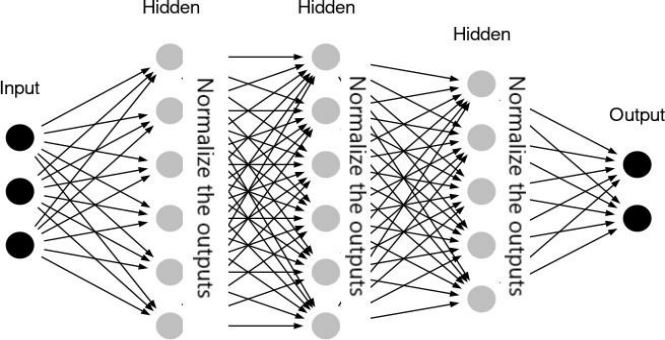
\includegraphics[height=2.25in]{batchnormalization1}
		\caption[Batch normalization of hidden layers]{Batch normalization of hidden layers.}
		\label{fig:batchnormalization1}
	\end{figure}
 	\begin{figure}[h]
		\centering
		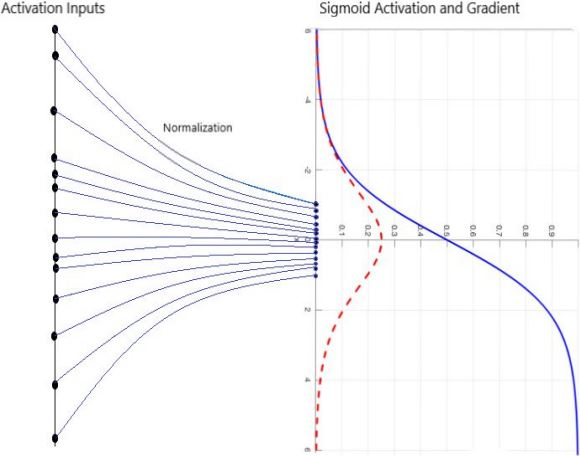
\includegraphics[height=2.25in]{batchnormalization2}
		\caption[Batch normalization and activation functions]{Batch normalization of a hidden layer's output to maps it to an appropriate range for an activation function.}
		\label{fig:batchnormalization2}
	\end{figure}

	\begin{equation}
		\hat{x}^k = \frac{x^k - E\left[x^k \right]}{\sqrt{Var\left[x^k \right]}}
		\label{eq:batchnormalization1}
	\end{equation}

	\subsection{Scale and Shift}
There are usually two stages in which Batch Normalization is applied:
	\begin{numberedlist}
		\item Before the activation function (non-linearity)
		\item After non-linearity
	\end{numberedlist}

	\vspace{\baselineskip}
	\begin{bulletedlist}
		\item For sigmoid and tanh activation, the normalized region is more linear than nonlinear.
		\item For ReLU activation, half of the inputs are zeroed out.
		\item So, some transformation has to be done to move the distribution away from 0.
		\item A scaling factor $\gamma$ and shifting factor $\beta$ are used to do this.
	\end{bulletedlist}

	\begin{equation}
		y^k = \gamma^k \hat{x}^k + \beta^k
		\label{eq:batchnormalization2}
	\end{equation}

	\subsection{Final Definition of Batch Normalization}
	\begin{numberedlist}
		\item Normalize using \equationname~\ref{eq:batchnormalization1}
		\item And then allow the network to squash the range if it wants to using \equationname~\ref{eq:batchnormalization2}, where $\gamma^k$ and $\beta^k$ are given by \equationname{}s~\ref{eq:batchnormalizationgamma} and~\ref{eq:batchnormalizationbeta}, respectively.
	\end{numberedlist}

	\begin{align}
		\gamma^k &= \sqrt{Var\left[x^k \right]} \label{eq:batchnormalizationgamma} \\
		\beta^k  &= E\left[x^k \right]          \label{eq:batchnormalizationbeta}
	\end{align}

	\subsection{Mini Batches}

	\begin{bulletedlist}
		\item Improves gradient flow through the network.
		\item Allows higher learning rates.
		\item Reduces the strong dependence on initialization.
		\item Acts as a form of regularization in a funny way, and slightly reduces the need for dropout, maybe.
	\end{bulletedlist}

	\vspace{\baselineskip}
	\begin{plainlist}
		\item {\bfseries Input}: Values of $x$ over a mini-batch $B = \{x_1 \ldots m \}$; parameters to be learned $\gamma, \beta$
		\item {\bfseries Output}: $\{ y_i = \textrm{B}\textrm{N}_{\gamma,\beta} \left(x_i\right) \}$
	\end{plainlist}

	\begin{align}
		\mu_B       &= \frac{1}{m} \sum_{i=1}^m x_i  \\
		\sigma_B^2  &= \frac{1}{m}  \sum_{i=1}^m \left( x_i - \mu_B \right)^2 \\
		\hat{x}_i   &= \frac{x_i - \mu_B}{\sqrt{\sigma_B^2 + \epsilon}}  \\
		y_i         &= \gamma\hat{x}_i + \beta \equiv \textrm{B}\textrm{N}_{\gamma,\beta} \left(x_i\right)
	\end{align}

	\subsubsection{Fitting the Batch Norm in the Deep Layers}
	\begin{bulletedlist}
		\item Batch Normalization is used on the input side just on the inputs of the layer before or after the activation function in the previous layer.
		\item It may be appropriate to use the Batch Normalization technique before the activation function for activations that may result in non-normal distributions like the ReLU activation function.
	\end{bulletedlist}

 	\begin{figure}[h]
		\centering
		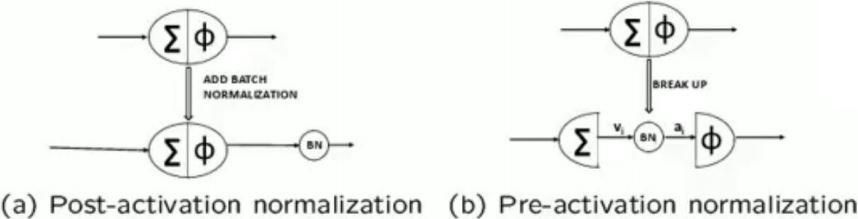
\includegraphics[height=1.25in]{batchnormalizationdeeplayers}
		\caption[Batch normalization of deep layers]{Batch normalization of deep layers.  In the above, $\phi$ is the activation function, $\sum$ is the summation of the inputs and weights, and BN is the batch normalization.}
		\label{fig:batchnormalizationdeeplayers}
	\end{figure}

	\subsubsection{Batch Normalization During Test Time}
	\begin{bulletedlist}
		\item Usually, when we use Batch Normalization, it is required to analyze its behavior during test time.  As the network gets trained, we try to normalize using population rather than using mini-batch statistics.
		\item Alternatively, we use the exponential moving average to compute the mean and variance for test time.
	\end{bulletedlist}


	\subsubsection{When Batch Normalization Does Not Work}
	\begin{bulletedlist}
		\item A feature of batch normalization in training mode changes the absolute scale of the features according to the batch statistics, which is a random variable, while the relative distances between features are preserved.
		\item This is completely fine for e.g. classification and segmentation tasks, where the semantics of the image are invariant to arbitrary scaling and shifting of the channel values.
		\item Batch normalization should not be used mostly with dropouts as dropouts shift the variance keeping the average constant.
For example, that you run a batch of images through batch normalization.  The absolute color information is lost, but the dogs will still look like dogs and cats will still look like cats.
		\item The information in the image data is preserved and the images can still be classified or segmented.
		\item In other words, in a dog/cat classification problem, as long as the features from an image of a dog remain more ``dog-like'' than ``cat-like'' after batch normalization, we do not worry too much about the absolute level of dog-likeness.
	\end{bulletedlist}

	\subsubsection{Guidelines for Batch Normalization}
	\begin{bulletedlist}
		\item Batch normalization may be used on the inputs to the layer before or after the activation function in the previous layer.
		\item It may be more appropriate after the activation function if for s-shaped functions like the hyperbolic tangent and logistic function.
		\item It may be appropriate before the activation function for activations that may result in non-Gaussian distributions like the rectified linear activation function, the modern default for most network types.
		\item Using batch norm depends on the problem, it should be used when the absolute scale of the features do not matter.
		\item Batch normalization should be used in the deeper network.
		\item Batch normalization often leads to a worse performance when It is combined with dropout in both theoretical and statistical aspects.
		\item Theoretically, dropout shifts the variance of a specific neural unit when we transfer the state of that network from train to test.
		\item However, batch normalization would maintain its statistical variance, which is accumulated from the entire learning procedure, in the test phase.
		\item The inconsistency of that variance (we name this scheme as ``variance shift'') causes the unstable numerical behavior in an inference that leads to more erroneous predictions finally when applying dropout before batch normalization.
	\end{bulletedlist}

	\section{Hyperparameter Optimization}
	\begin{bulletedlist}
		\item Parameters are the ones which the model will learn from the data and gives the values.  Examples:
		\begin{bulletedlist}
			\item In Linear regression, the weight coefficients and bias are learned from the data.
			\item In the Support Vector Machine, support vectors near the margin line are parameters.
		\end{bulletedlist}
		\item Hyperparameters are the ones which we will be giving the model that helps in the learning process.  Examples:
		\begin{bulletedlist}
			\item In Decision Tree and Random Forest max\_Depth, min\_sample, min\_sample\_leaf, max\_leaf\_node, and criterion are the hyperparameters.
		\end{bulletedlist}
	\end{bulletedlist}

	\vspace{\baselineskip}
	\begin{bulletedlist}
		\item Hyperparameters in neural networks include:
		\begin{bulletedlist}
			\item Activation Function
			\item Number of Neurons in each layer
			\item Number of hidden layers
			\item Optimizer
			\item Loss/cost function
		\end{bulletedlist}
		\item Hyperparameters to play with:
		\begin{bulletedlist}
			\item Network architecture
			\item Learning rate, its multiplier schedule
			\item Regularization (L2/dropout strength)
		\end{bulletedlist}
	\end{bulletedlist}

 	\begin{figure}[h]
		\centering
		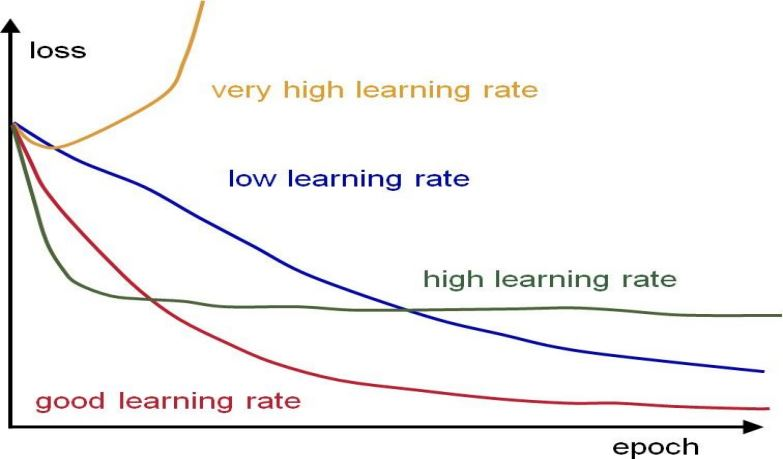
\includegraphics[height=1.8in]{neuralnetworklearningrates}
		\caption[Learning rates in neural networks]{Learning rates in neural networks.}
		\label{fig:neuralnetworklearningrates}
	\end{figure}

 	\begin{figure}[h]
		\centering
		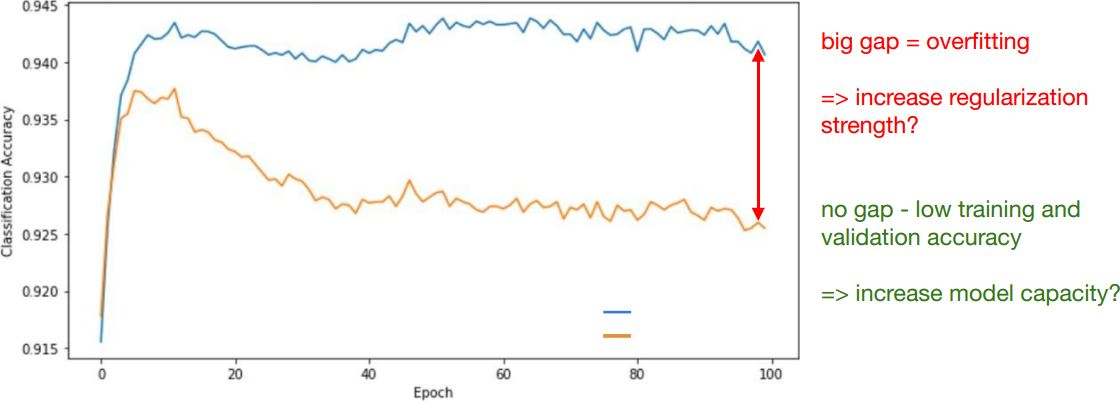
\includegraphics[height=1.8in]{neuralnetworkslosscurve}
		\caption[Loss curve in neural networks]{Loss curve in neural networks.  Training curve is in blue, validation curve is in gold.}
		\label{fig:neuralnetworkslosscurve}
	\end{figure}

	\section{Recipe for Training Neural Network}
	\begin{numberedlist}
		\item Become one with the data.
		\item Set up the end-to-end training/evaluation skeleton + get dumb baselines.
		\item Over fit.
		\item Regularize.
		\item Tune.
		\item Squeeze out the juice.
	\end{numberedlist}

	\section{Types of Neural Networks}
	\begin{bulletedlist}
		\item Feed forward.
		\begin{bulletedlist}
			\item Information is only fed forward.
			\item Multi-layer perceptron.
			\item Convolution neural networks.
			\begin{bulletedlist}
				\item Popular in computer vision.
				\item Builds nodes in grids.
				\item Feeds information to nodes from overlapping grids.
				\item After a few layers of grids, the information gets flatten to an array and fed into a normal neural network.
				\item Helps to keep spacial information.
			\end{bulletedlist}
		\end{bulletedlist}
		\item Recurrent neural networks.
		\begin{bulletedlist}
			\item Good for time series data.
			\item Uses some sense of memory, what happens next depends on some way what happened in the past.
			\item Nodes can get input from previous runs (see \equationname{}s~\ref{eq:recurrentneuralnetwork1} and~\ref{eq:recurrentneuralnetwork2}).
			\item
			\item LSTM (long short term memories).
			\begin{bulletedlist}
				\item Replaces node with algorithm/node that remembers more history.
			\end{bulletedlist}
		\end{bulletedlist}
		\item Deep neural networks.
		\begin{bulletedlist}
			\item Networks with many layers.  There is no formal definition of how many layers is needed to qualify as a deep network.
		\end{bulletedlist}
		\item GAN (generalized adversarial networks).
		\begin{bulletedlist}
			\item Two neural networks working and testing off of each other.
			\item One network creates input for the other.
			\item Second network is called the discriminator.
		\end{bulletedlist}
	\end{bulletedlist}

	\begin{align}
		w_1 x^1 + w_2 x^2            &= z  \label{eq:recurrentneuralnetwork1} \\
		w_1 x^1 + w_2 x^2 + z^{old}  &= z  \label{eq:recurrentneuralnetwork2}
	\end{align}

	\section{Hands On Neural Network} 